%
\begin{isabellebody}%
\def\isabellecontext{Hanoi}%
\isamarkupfalse%
%
\isamarkupsubsection{The towers of Hanoi \label{psv2000hanoi}%
}
\isamarkuptrue%
%
\begin{isamarkuptext}%
We are given 3 pegs $A$, $B$ and $C$, and $n$ disks with a hole, such
that no two disks have the same diameter.  Initially all $n$ disks
rest on peg $A$, ordered according to their size, with the largest one
at the bottom. The aim is to transfer all $n$ disks from $A$ to $C$ by
a sequence of single-disk moves such that we never place a larger disk
on top of a smaller one. Peg $B$ may be used for intermediate storage.

\begin{center}
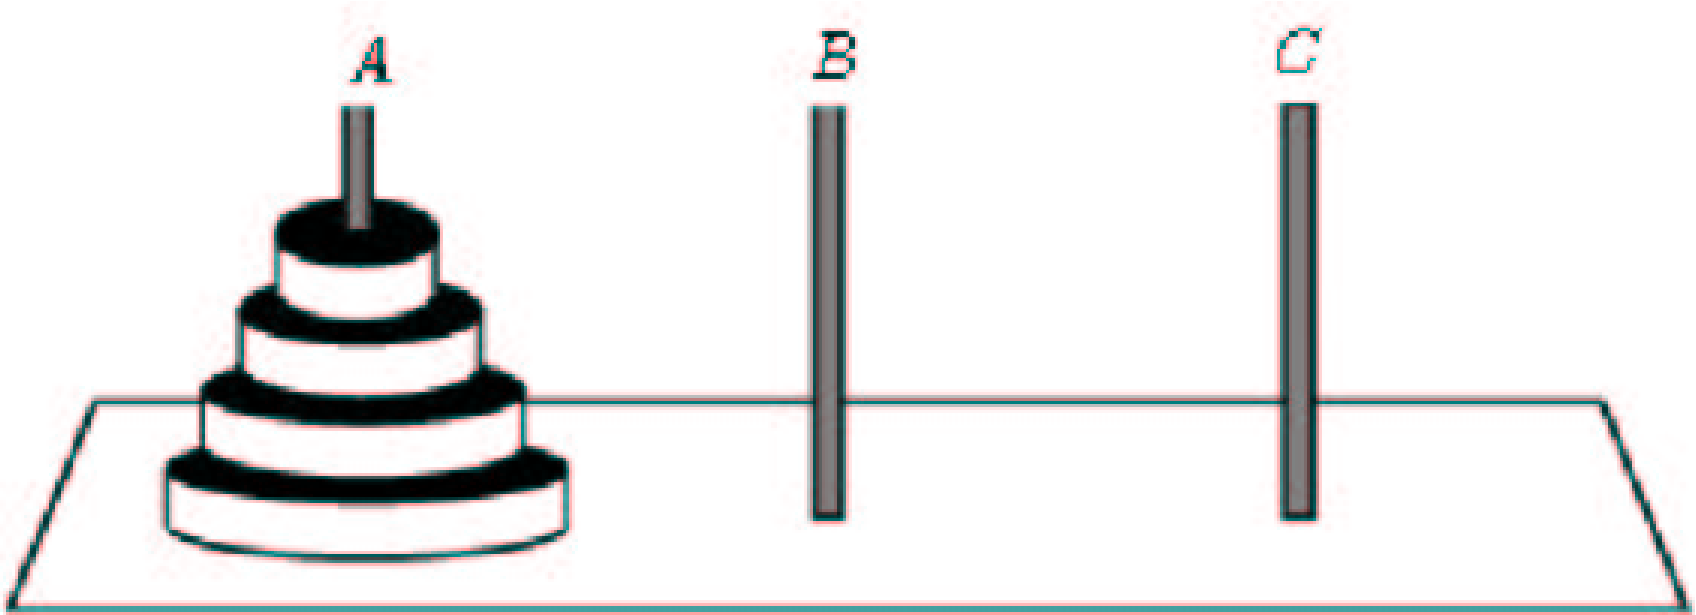
\includegraphics[width=0.8\textwidth]{Hanoi}
\end{center}

\medskip The pegs and moves can be modelled as follows:%
\end{isamarkuptext}%
\isamarkuptrue%
\isacommand{datatype}\ peg\ {\isacharequal}\ A\ {\isacharbar}\ B\ {\isacharbar}\ C\isanewline
\isamarkupfalse%
\isacommand{types}\ move\ {\isacharequal}\ {\isachardoublequote}peg\ {\isacharasterisk}\ peg{\isachardoublequote}\isamarkupfalse%
%
\begin{isamarkuptext}%
Define a primitive recursive function%
\end{isamarkuptext}%
\isamarkuptrue%
\isacommand{consts}\isanewline
\ \ moves\ {\isacharcolon}{\isacharcolon}\ {\isachardoublequote}nat\ {\isacharequal}{\isachargreater}\ peg\ {\isacharequal}{\isachargreater}\ peg\ {\isacharequal}{\isachargreater}\ peg\ {\isacharequal}{\isachargreater}\ move\ list{\isachardoublequote}\isamarkupfalse%
%
\begin{isamarkuptext}%
such that \isa{moves}$~n~a~b~c$ returns a list of (legal)
moves that transfer $n$ disks from peg $a$ via $b$ to $c$.
Show that this requires $2^n - 1$ moves:%
\end{isamarkuptext}%
\isamarkuptrue%
\isacommand{theorem}\ {\isachardoublequote}length\ {\isacharparenleft}moves\ n\ a\ b\ c{\isacharparenright}\ {\isacharequal}\ {\isadigit{2}}{\isacharcircum}n\ {\isacharminus}\ {\isadigit{1}}{\isachardoublequote}\isamarkupfalse%
\isamarkupfalse%
%
\begin{isamarkuptext}%
Hint: You need to strengthen the theorem for the
induction to go through. Beware: subtraction on natural numbers
behaves oddly: $n - m = 0$ if $n \le m$.%
\end{isamarkuptext}%
\isamarkuptrue%
\isamarkupfalse%
\end{isabellebody}%
%%% Local Variables:
%%% mode: latex
%%% TeX-master: "root"
%%% End:
